\documentclass{standalone}
\usepackage{amsmath}
\usepackage{tikz}
\usepackage{rotating}
\usetikzlibrary{shapes.geometric, arrows.meta}

\tikzstyle{process} = [rectangle, 
minimum width=3cm, 
minimum height=1cm, 
text centered,  
draw=black, 
fill=orange!30]

\begin{document}

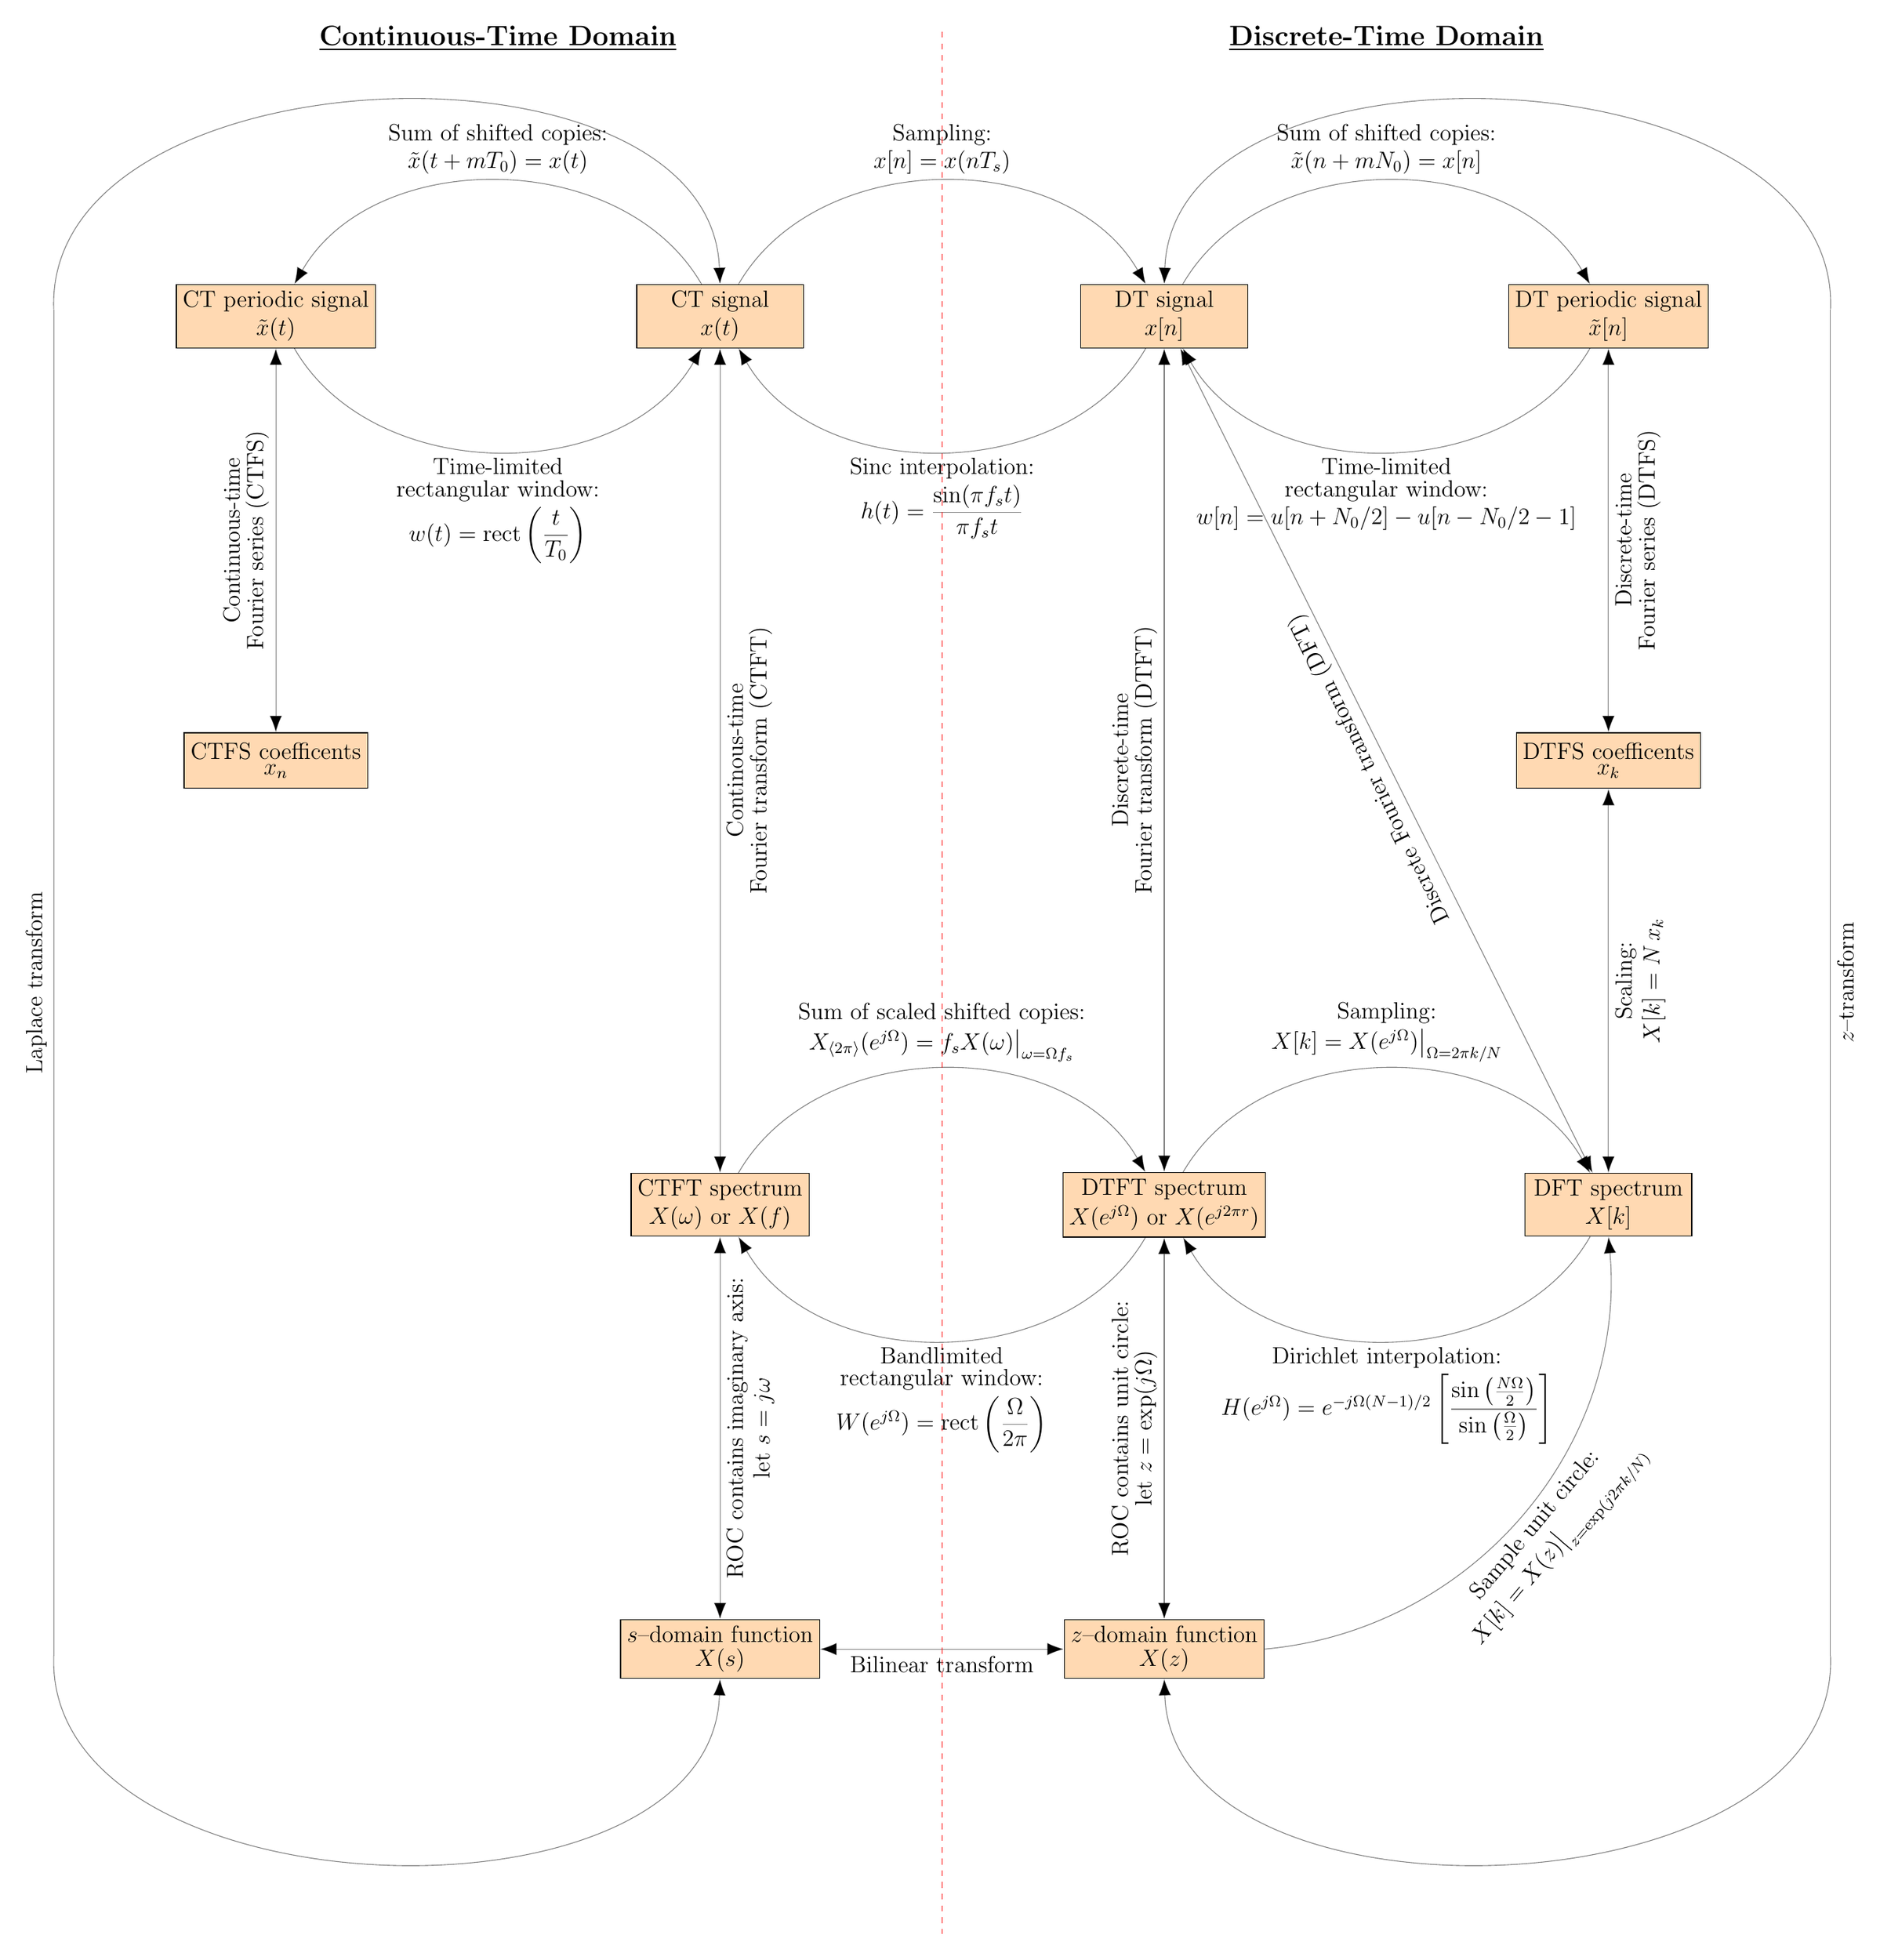
\begin{tikzpicture}[node distance=2cm]

\node (ct) [process] {\large\shortstack{CT signal\\$x(t)$}};
\node (dt) [process, right of=ct, xshift=6cm] {\large\shortstack{DT signal\\$x[n]$}};
\draw[-{Latex[length=3mm]}, draw opacity=0.5] (ct) to[bend right=-60] node[midway,above] {\large\shortstack{Sampling:\\$x[n]=x(nT_s)$}} (dt);
\draw[-{Latex[length=3mm]}, draw opacity=0.5] (dt) to[bend left=60] node[midway,below] {\large\shortstack{Sinc interpolation:\\$h(t)=\dfrac{\sin(\pi f_s t)}{\pi f_s t}$}} (ct);

\node (pct) [process, left of=ct, xshift=-6cm] {\large\shortstack{CT periodic signal\\$\tilde{x}(t)$}};
\draw[-{Latex[length=3mm]}, draw opacity=0.5] (ct) to[bend left=-60] node[midway,above] {\large\shortstack{Sum of shifted copies:\\$\tilde{x}(t + mT_0) = x(t)$}} (pct);
\draw[-{Latex[length=3mm]}, draw opacity=0.5] (pct) to[bend right=60] node[midway,below] {\large\shortstack{Time-limited\\rectangular window:\\$w(t)=\operatorname{rect}\left(\dfrac{t}{T_0}\right)$}} (ct);
\node (pdt) [process, right of=dt, xshift=6cm] {\large\shortstack{DT periodic signal\\$\tilde{x}[n]$}};
\draw[-{Latex[length=3mm]}, draw opacity=0.5] (dt) to[bend right=-60] node[midway,above] {\large\shortstack{Sum of shifted copies:\\$\tilde{x}(n + mN_0) = x[n]$}} (pdt);
\draw[-{Latex[length=3mm]}, draw opacity=0.5] (pdt) to[bend left=60] node[midway,below] {\large\shortstack{Time-limited\\rectangular window:\\$w[n]=u[n+N_0/2]-u[n-N_0/2-1]$}} (dt);

\node (ctfs) [process, below of=pct, yshift=-6cm] {\large\shortstack{CTFS coefficents\\$x_n$}};
\draw[{Latex[length=3mm]}-{Latex[length=3mm]}, draw opacity=0.5] (pct) to node[above,midway,rotate=90] {\large\shortstack{Continuous-time\\Fourier series (CTFS)}} (ctfs);

\node (dtfs) [process, below of=pdt, yshift=-6cm] {\large\shortstack{DTFS coefficents\\$x_k$}};
\draw[{Latex[length=3mm]}-{Latex[length=3mm]}, draw opacity=0.5] (pdt) to node[below,midway,rotate=90] {\large\shortstack{Discrete-time\\Fourier series (DTFS)}} (dtfs);
\node (dft) [process, below of=dtfs, yshift=-6cm] {\large\shortstack{DFT spectrum\\$X[k]$}};
\draw[{Latex[length=3mm]}-{Latex[length=3mm]}, draw opacity=0.5] (dft) to node[below,midway,rotate=90] {\large\shortstack{Scaling:\\$X[k]=N\,x_k$}} (dtfs);

\node (dtft) [process, left of=dft, xshift=-6cm] {\large\shortstack{DTFT spectrum\\$X(e^{j\Omega})$ or $X(e^{j2\pi r})$}};
\draw[-{Latex[length=3mm]}, draw opacity=0.5] (dtft) to[bend right=-60] node[midway,above] {\large\shortstack{Sampling:\\$X[k] = X(e^{j\Omega})\big|_{\Omega=2\pi k/N}$}} (dft);
\draw[-{Latex[length=3mm]}, draw opacity=0.5] (dft) to[bend left=60] node[midway,below] {\large\shortstack{Dirichlet interpolation:\\$H(e^{j\Omega})=e^{-j\Omega(N-1)/2}\left[\dfrac{\sin\left(\frac{N\Omega}{2}\right)}{\sin\left(\frac{\Omega}{2}\right)}\right]$}} (dtft);
\draw[{Latex[length=3mm]}-{Latex[length=3mm]}, draw opacity=0.5] (dt) to node[above,midway,rotate=90] {\large\shortstack{Discrete-time\\Fourier transform (DTFT)}} (dtft);

\node (ctft) [process, left of=dtft, xshift=-6cm] {\large\shortstack{CTFT spectrum\\$X(\omega)$ or $X(f)$}};
\draw[-{Latex[length=3mm]}, draw opacity=0.5] (ctft) to[bend right=-60] node[midway,above] {\large\shortstack{Sum of scaled shifted copies:\\$X_{\langle 2\pi\rangle}(e^{j\Omega}) = f_s X(\omega)\big|_{\omega=\Omega f_s}$}} (dtft);
\draw[-{Latex[length=3mm]}, draw opacity=0.5] (dtft) to[bend left=60] node[midway,below] {\large\shortstack{Bandlimited\\rectangular window:\\$W(e^{j\Omega})=\operatorname{rect}\left(\dfrac{\Omega}{2\pi}\right)$}} (ctft);
\draw[{Latex[length=3mm]}-{Latex[length=3mm]}, draw opacity=0.5] (ct) to node[below,midway,rotate=90] {\large\shortstack{Continous-time\\Fourier transform (CTFT)}} (ctft);

\draw[{Latex[length=3mm]}-{Latex[length=3mm]}, draw opacity=0.5] (dt) to node[above,midway,rotate=116] {\large Discrete Fourier transform (DFT)} (dft);

\node (laplace) [process, below of=ctft, yshift=-6cm] {\large\shortstack{$s$--domain function\\$X(s)$}};
\draw[{Latex[length=3mm]}-{Latex[length=3mm]}, draw opacity=0.5] (laplace) to node[below,midway,rotate=90] {\large\shortstack{ROC contains imaginary axis:\\let $s=j\omega$}} (ctft);

\node (z_tr) [process, below of=dtft, yshift=-6cm] {\large\shortstack{$z$--domain function\\$X(z)$}};
\draw[{Latex[length=3mm]}-{Latex[length=3mm]}, draw opacity=0.5] (z_tr) to node[above,midway,rotate=90] {\large\shortstack{ROC contains unit circle:\\let $z=\exp(j\Omega)$}} (dtft);
\draw[{Latex[length=3mm]}-{Latex[length=3mm]}, draw opacity=0.5] (z_tr) to node[below,midway] {\large Bilinear transform} (laplace);
\draw[-{Latex[length=3mm]}, draw opacity=0.5] (z_tr) to[bend right=45] node[below,midway,rotate=50] {\large\shortstack{Sample unit circle:\\$X[k]=X(z)\big|_{z=\exp(j2\pi k/N)}$}} (dft);

\node (pt1) [left of=pct, xshift=-2cm] {}; 
\node (pt2) [below of=pt1, yshift=-22cm] {}; 
\draw[-, draw opacity=0.5] (pt1.north) to node[above,midway,rotate=90] {\large Laplace transform} (pt2.south);
\draw[-{Latex[length=3mm]}, draw opacity=0.5] (pt1) to[bend left=90] (ct);
\draw[-{Latex[length=3mm]}, draw opacity=0.5] (pt2) to[bend left=-90] (laplace);

\node (pt3) [right of=pdt, xshift=2cm] {}; 
\node (pt4) [below of=pt3, yshift=-22cm] {}; 
\draw[-, draw opacity=0.5] (pt3.north) to node[below,midway,rotate=90] {\large $z$--transform} (pt4.south);
\draw[-{Latex[length=3mm]}, draw opacity=0.5] (pt3) to[bend right=90] (dt);
\draw[-{Latex[length=3mm]}, draw opacity=0.5] (pt4) to[bend right=-90] (z_tr);

\node (pt5) [right of=ct, xshift=2cm, yshift=5cm] {}; 
\node (pt6) [below of=pt5, yshift=-32cm] {}; 
\draw[dashed, red, draw opacity=0.5] (pt5.north) to (pt6.south);

\node[left of=pt5, xshift=-6cm] {\Large\textbf{\underline{Continuous-Time Domain}}}; 
\node[right of=pt5, xshift=6cm] {\Large\textbf{\underline{Discrete-Time Domain}}}; 

\end{tikzpicture}
\end{document}